
% Template for Project Solutions
% Research Group for Parallel Computing
% Vienna University of Technology

% Copyright (C) 2017
% Sascha Hunold <hunold@par.tuwien.ac.at>
% version 1.0.0

\documentclass[DIV12,a4paper]{scrartcl}

\usepackage[utf8]{inputenc}
\usepackage[T1]{fontenc}

\usepackage{amsmath}  
\usepackage{amssymb} 
\usepackage{microtype} 
\usepackage{booktabs} 
\usepackage{nag}       % Issues warnings when best practices in writing LaTeX documents are violated.
\usepackage{hyperref}
\usepackage{xspace}
\usepackage{graphicx}
\usepackage[square,numbers]{natbib}  % need this for DOI (or use biber/biblatex)

%%%%%%%%%%%%%%%%%%%%%%%%%%%%%%%%%%%
% ONLY CHANGE THE FOLLOWING MACROS

\newcommand{\studnameA}{Philipp Paris}
\newcommand{\studemailA}{e1325664@student.tuwien.ac.at}
\newcommand{\studmatrikelA}{1325664}

\newcommand{\studnameB}{Emmanuel Pescosta}
\newcommand{\studemailB}{e1326934@student.tuwien.ac.at}
\newcommand{\studmatrikelB}{1326934}

% name of class
\newcommand{\coursename}{High Performance Computing}
%\newcommand{\coursename}{Advanced Multiprocessor Programming}
%\newcommand{\coursename}{Parallel Algorithms}

\newcommand{\coursesemester}{SS 2017}

\newcommand{\projectname}{Project 2}

% date when you hand in 
\newcommand{\projectdate}{12 June 2017}


% YOU SHOULD NOT NEED TO CHANGE THE REMAINING FILE
%%%%%%%%%%%%%%%%%%%%%%%%%%%%%%%%%%%

\graphicspath{{graphics/}}

\begin{document}

\pagenumbering{Alph} % remove some hyperref warning
% !TEX root = template.tex

\pagestyle{empty}

\begin{titlepage}
\begin{center}

\includegraphics[scale=1]{TU_INF_Logo_gray}
\hfill

\includegraphics[width=1.7cm]{final-logo-par}

\end{center}

\vspace*{1cm}

\begin{center}

\vspace{3cm}

\begin{Huge}
\textbf{Project Report}\\
\end{Huge}

\vspace{1ex}

{\large{} for}

\vspace{1ex}

\begin{huge}
\textbf{\projectname{}}
\end{huge}

\vspace*{1cm}

as part of VU on

\begin{Large}
\coursename{}\\[1ex]
\coursesemester
\end{Large}


\vspace*{2cm}


\vspace*{1cm}

\begin{Large}
\studnameA \\
\texttt{\studemailA} \\
\studmatrikelA\\[1cm]

\studnameB \\
\texttt{\studemailB} \\
\studmatrikelB\\[1cm]

\vspace*{1cm}
\projectdate \\

\end{Large}
\end{center}

\end{titlepage}


\cleardoublepage
\pagenumbering{arabic}
\pagestyle{plain}

\setcounter{page}{1}

% !TEX root = template.tex

\newcommand\mygather{\texttt{MY\_Gather}\xspace}
\newcommand\myscatter{\texttt{MY\_Scatter}\xspace}

\newcommand\mpigather{\texttt{MPI\_Gather}\xspace}
\newcommand\mpiscatter{\texttt{MPI\_Scatter}\xspace}

%----------------------------------------------------------------------
\section{Algorithm \mygather}

%-------
\subsection{Strategy Comparison}

Two different \texttt{Gather} algorithms, one based on Binomial-Trees and one based on a Divide-And-Conquer approach were implemented and tested. Both algorithms fulfill the specification of \mpigather and use the minimum amount of memory whenever possible. Figure \ref{fig:gather:binom_vs_dac:root0} shows the performance of each implementation compared to the \texttt{Open MPI Gather} implementation with $root = 0$. Figure \ref{fig:gather:binom_vs_dac:root2} shows the same comparison with $root = 2$.

\begin{figure}[H]
  \centering
  \begin{subfigure}[b]{0.49\textwidth}
        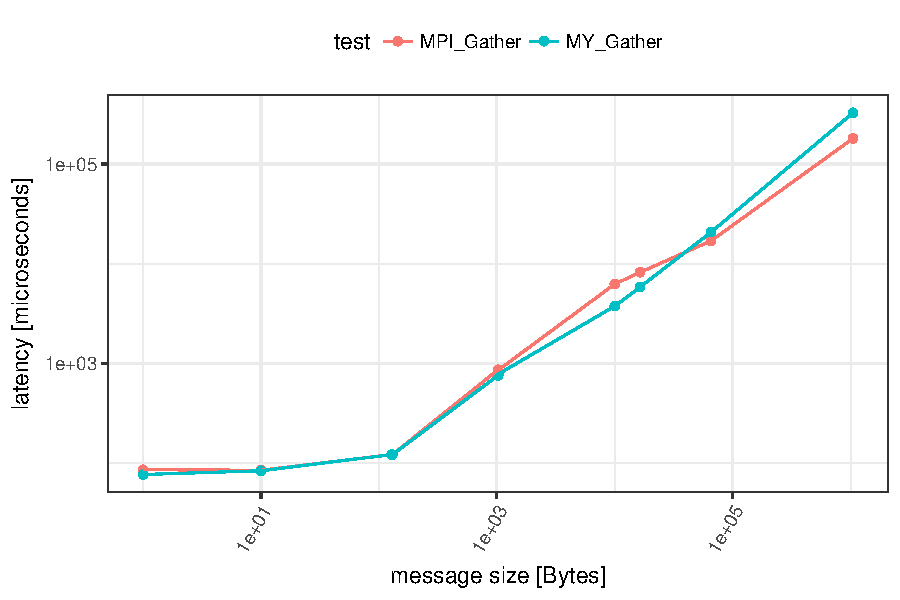
\includegraphics[width=\textwidth]{../benchmarks/openmpi/binom/gather_32/runtime.pdf}
        \caption{Binomial-Tree Implementation}
    \end{subfigure}
    \begin{subfigure}[b]{0.49\textwidth}
        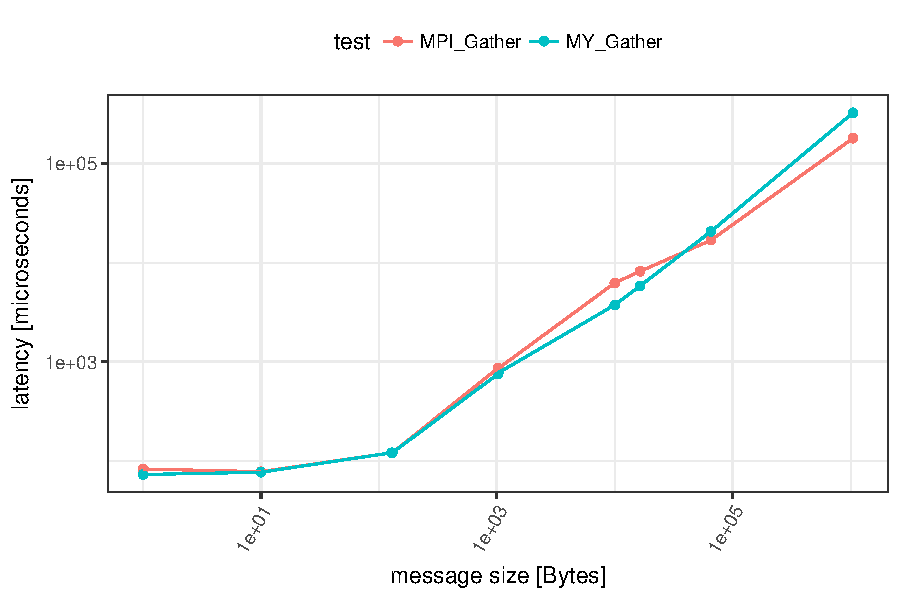
\includegraphics[width=\textwidth]{../benchmarks/openmpi/divide_conquer/gather32/runtime.pdf}
        \caption{Divide-And-Conquer Implementation}
    \end{subfigure}
    \caption{Binomial Tree and Divide-And-Conquer \texttt{Gather} with $root = 0$}
    \label{fig:gather:binom_vs_dac:root0}
\end{figure}

\begin{figure}[H]
  \centering
  \begin{subfigure}[b]{0.49\textwidth}
        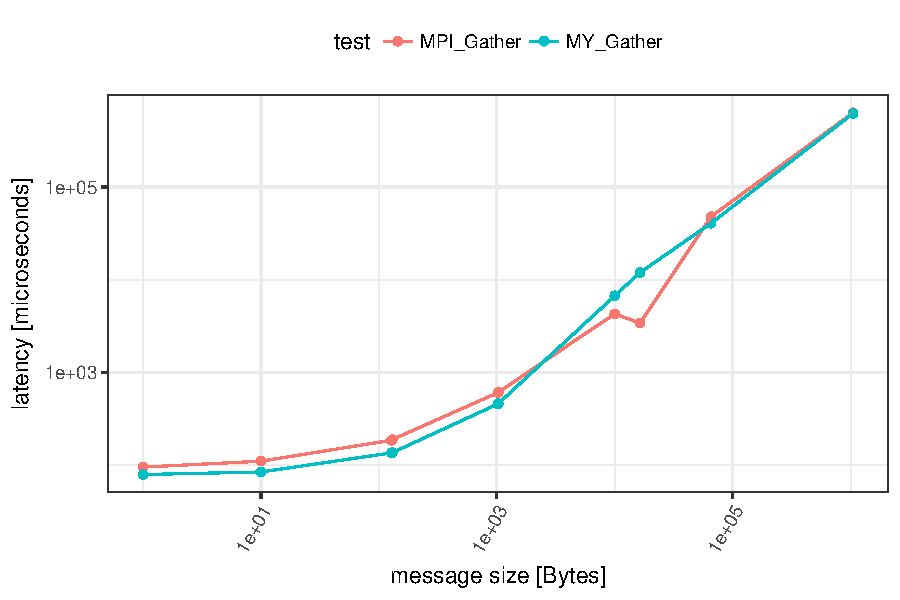
\includegraphics[width=\textwidth]{../benchmarks/openmpi/root=2/binom/gather_32/runtime.pdf}
        \caption{Binomial-Tree Implementation}
    \end{subfigure}
    \begin{subfigure}[b]{0.49\textwidth}
        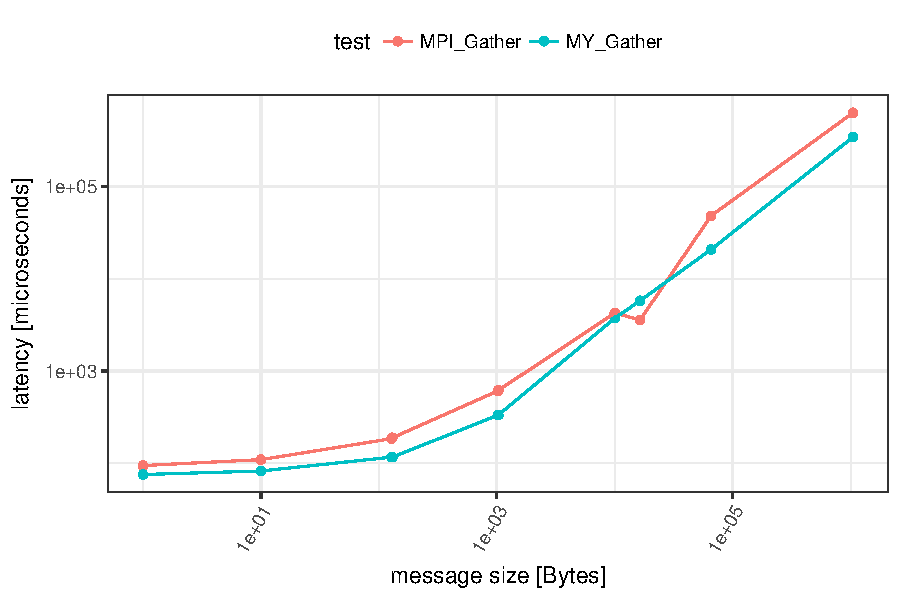
\includegraphics[width=\textwidth]{../benchmarks/openmpi/root=2/divide_conquer/gather_32/runtime.pdf}
        \caption{Divide-And-Conquer Implementation}
    \end{subfigure}
    \caption{Binomial Tree and Divide-And-Conquer \texttt{Gather} with $root = 2$}
    \label{fig:gather:binom_vs_dac:root2}
\end{figure}

\noindent As seen in Figure \ref{fig:gather:binom_vs_dac:root0}, both algorithms perform similarly when the root node has rank $0$. In this case the binomial-tree based algorithm directly receives into the \textit{recvbuf} without the need of expensive reordering. But when using rank $2$ as the root, the reordering of data in the Binomial-Tree implementation cannot be avoided and thus leads to an overhead. Therefore the Divide-And-Conquer algorithm performs better when rank $\neq 0$, as seen in Figure \ref{fig:gather:binom_vs_dac:root2}.\\
Because the following benchmarks are all done with $root = 0$, the binomial-tree implementation was chosen as the main strategy.

%-------
\subsection{Description / Strategy}

All processing nodes are organized in a binomial-tree with the root of the \texttt{Gather} algorithm as the root of the tree. Each leaf node sends its data to its parent node and all non-leaf nodes forward all received data as well as the local data of the node itself to the parent. \\
Due to the use of a binomial tree, the calculation of the parent and child ranks can be done via fast bit-operations.\\

\noindent For cases where the root node has $rank \neq 0$, the algorithm uses virtual ranks:
$vrank = (rank - root - N ) \mod N$. In this case the data is received in virtual rank order at the root and has to be reordered to regain the real rank order.\\

\noindent To reduce the memory footprint of the algorithm, each node determines the expected amount of data it needs to store in the temporary buffer. Leaf nodes don't require any temporary buffer. For the root node the number of expected blocks, where a block is the amount of data of a single node, is equal to the the number of the nodes in the communicator. Each forwarding node (non-leaf and non-root nodes) can simply calculate the amount of expected blocks by taking the minimum of 
$2^{count\_zeros(vrank)}$ and $size - vrank$.

\subsection{Round- and Bandwidth Optimality}

\subsubsection{Round Optimality}
Due to the tree structure nodes on the same level send data to their parent nodes in parallel, so each layer of the tree represents one communication round. Therefore the number of communications rounds is limited by $\mathcal{O}(log(p))$.

\subsubsection{Bandwidth Optimality}
When m is the total amount of data to be gathered, then every process sends and receives $\frac{m}{p}$ units of data at every step. The algorithm takes $p-1$ steps to complete, and therefore the bandwidth term is $\frac{p-1}{p} m \beta$.\\
This cannot be reduced because the root node has to receive $\frac{m}{p}$ units of data from $p-1$ processes.

%-------
\subsection{Harmful Algorithmic Latency}
No Algorithmic Latency: Due to the calculation of child and parent nodes via bit operations, each processor can start to send/receive after $\mathcal{O}(1)$ steps.


%----------------------------------------------------------------------
\section{Algorithm \myscatter}

%-------
\subsection{Strategy Comparison}
Again two \texttt{Scatter} algorithms one based on Binomial-Trees and one based on Divide-And-Conquer were implemented and compared. Both algorithms fulfill the specification of \mpigather and use the minimum amount of memory whenever possible. Figure \ref{fig:scatter:binom_vs_dac:root0} shows the performance of each implementation compared to the \texttt{Open MPI Scatter} implementation with $root = 0$. Figure \ref{fig:scatter:binom_vs_dac:root2} shows the same comparison with $root = 2$.

\begin{figure}[H]
  \centering
  \begin{subfigure}[b]{0.49\textwidth}
        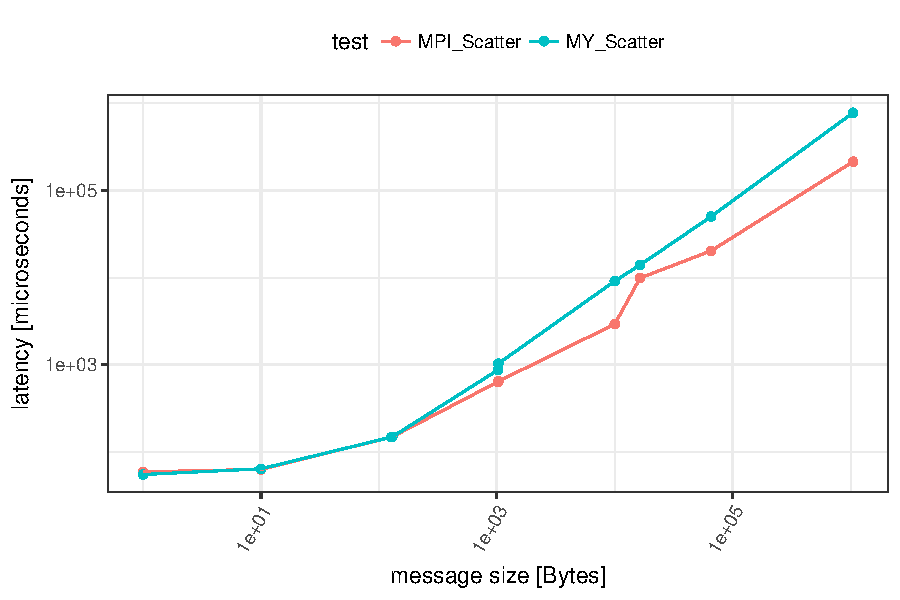
\includegraphics[width=\textwidth]{../benchmarks/openmpi/binom/scatter_32/runtime.pdf}
        \caption{Binomial-Tree Implementation}
    \end{subfigure}
    \begin{subfigure}[b]{0.49\textwidth}
        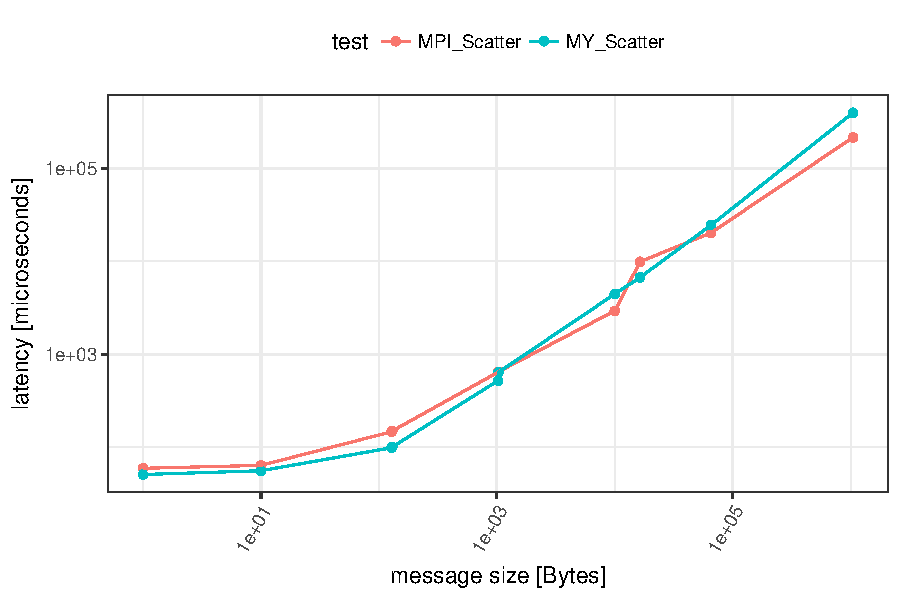
\includegraphics[width=\textwidth]{../benchmarks/openmpi/divide_conquer/scatter_32/runtime.pdf}
        \caption{Divide-And-Conquer Implementation}
    \end{subfigure}
    \caption{Binomial Tree and Divide-And-Conquer \texttt{Scatter} with $root = 0$}
    \label{fig:scatter:binom_vs_dac:root0}
\end{figure}

\begin{figure}[H]
  \centering
  \begin{subfigure}[b]{0.49\textwidth}
        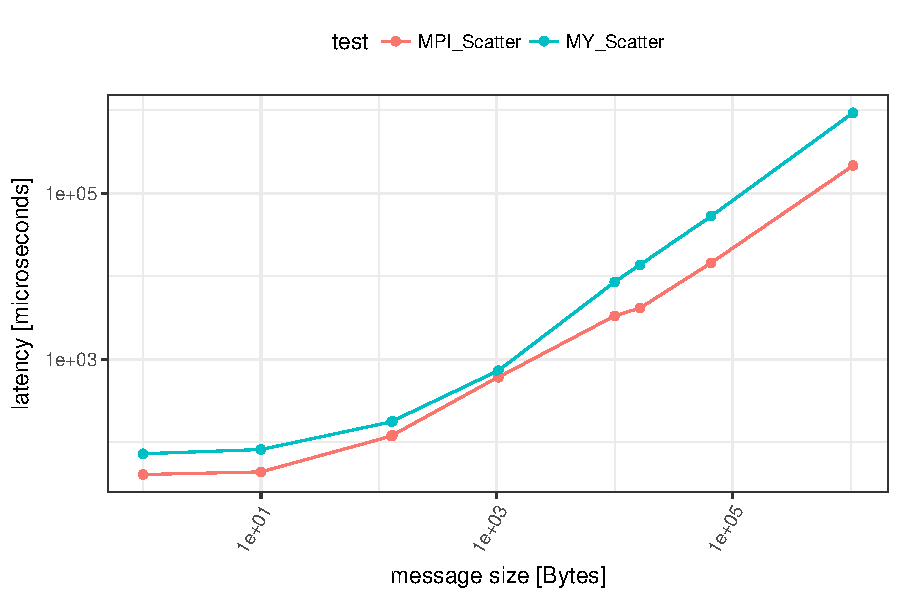
\includegraphics[width=\textwidth]{../benchmarks/openmpi/root=2/binom/scatter_32/runtime.pdf}
        \caption{Binomial-Tree Implementation}
    \end{subfigure}
    \begin{subfigure}[b]{0.49\textwidth}
        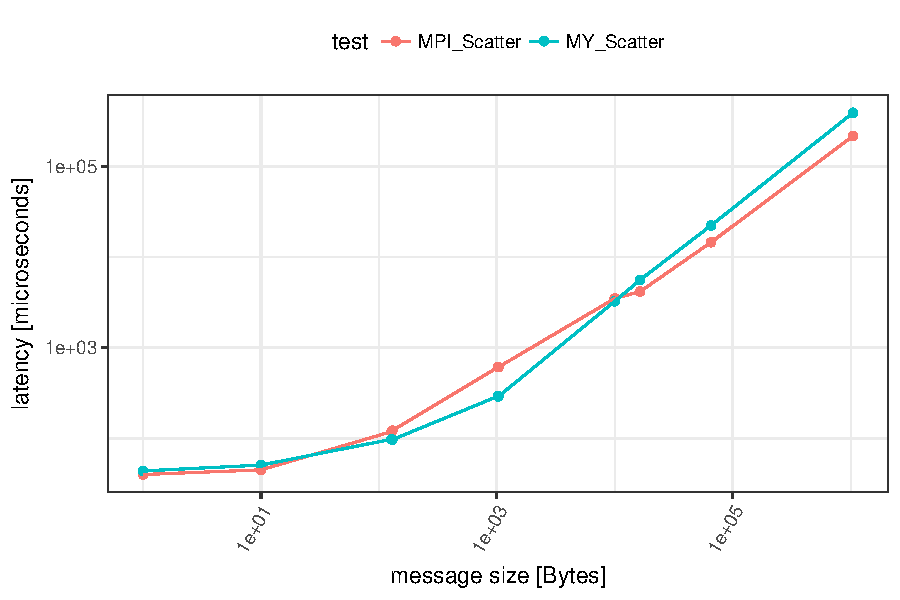
\includegraphics[width=\textwidth]{../benchmarks/openmpi/root=2/divide_conquer/scatter_32/runtime.pdf}
        \caption{Divide-And-Conquer Implementation}
    \end{subfigure}
    \caption{Binomial Tree and Divide-And-Conquer \texttt{Scatter} with $root = 2$}
    \label{fig:scatter:binom_vs_dac:root2}
\end{figure}

\noindent As before, the performance of the Binomial-Tree algorithm performs worse than the Divide-And-Conquer approach when using $rank \neq 0$, due to the reordering overhead on the \texttt{Scatter} root node. Also the Divide-And-Conquer algorithm performs better for medium and big message sizes.\\
Due to the better overall performance of the Divide-And-Conquer based algorithm, this implementation was  chosen as baseline implementation for the following discussions.


%-------
\subsection{Description / Strategy}

Divide-And-Conquer works by recursively breaking down a given problem into a number of sub-problems, in this case two sub-problems. The processes are split into two sets and the root nodes selects one process, denoted as \textit{subroot}, from the other set and sends half of the data to it. This is repeated for both sets until every node has received its data. On each communication round the number of senders is increased by a factor of two, while the amount of data to be send on each node is decreased by a factor of two.\newline

\noindent Cases where the \texttt{Scatter} root node has $rank \neq 0$ are already covered by this algorithm and thus don't require additional efforts. 

%-------
\subsection{Round- and Bandwidth Optimality}

\subsubsection{Round Optimality}

Using the Divide-And-Conquer approach, the data is distributed to the nodes along a binary tree, where all communication on the same tree-layer is executed at the same time. Therefore the number of communication rounds is limited by $\mathcal{O}(log(p))$.

\subsubsection{Bandwidth Optimality}

The root node has to send $\frac{m}{p}$ units of data to $p-1$ processes and therefore the bandwidth term for the Divide-And-Conquer Scatter is $\frac{p-1}{p} m \beta$.

%-------
\subsection{Harmful Algorithmic Latency}

No Algorithmic Latency: Each processor can start to send/receive after $\mathcal{O}(1)$ steps.

%----------------------------------------------------------------------
\section{Experimental Results}

%-------
\subsection{Experiments and Discussion -- \mygather}

\begin{figure}[H]
    \centering
    
    \begin{subfigure}[b]{0.49\textwidth}
        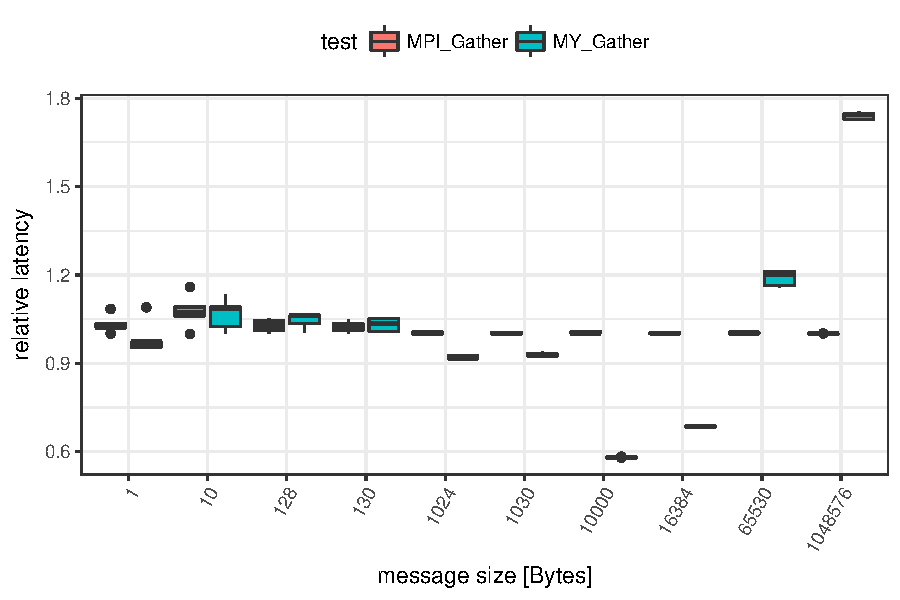
\includegraphics[width=\textwidth]{../benchmarks/openmpi/binom/gather_31/rel_runtime.pdf}
        \caption{Relative Runtime with $p=31 \times 16$}
        \label{fig:Gather:OpenMPI:Rel:31}
    \end{subfigure}
    \begin{subfigure}[b]{0.49\textwidth}
        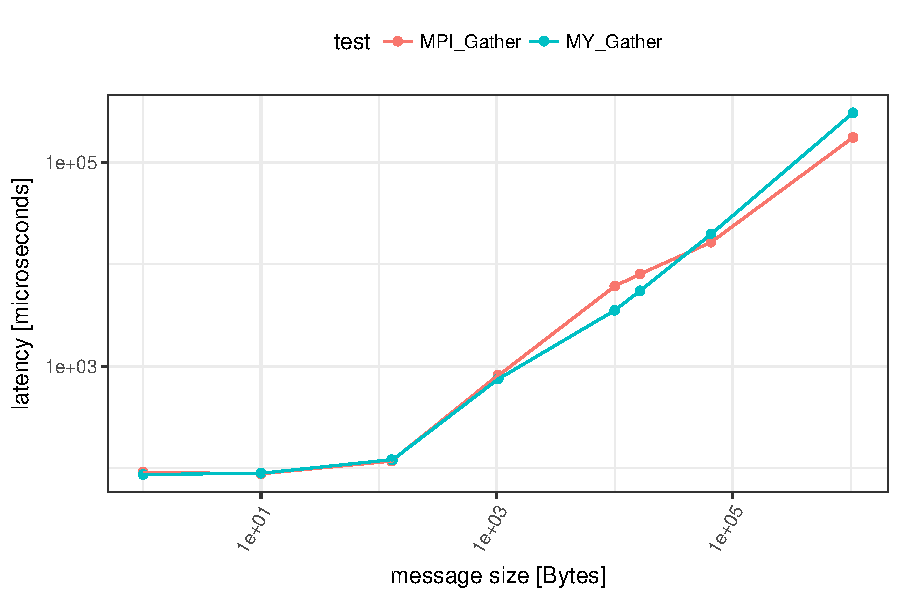
\includegraphics[width=\textwidth]{../benchmarks/openmpi/binom/gather_31/runtime.pdf}
        \caption{Absolute Runtime with $p=31 \times 16$}
        \label{fig:Gather:OpenMPI:Abs:31}
    \end{subfigure}
    
    \begin{subfigure}[b]{0.49\textwidth}
        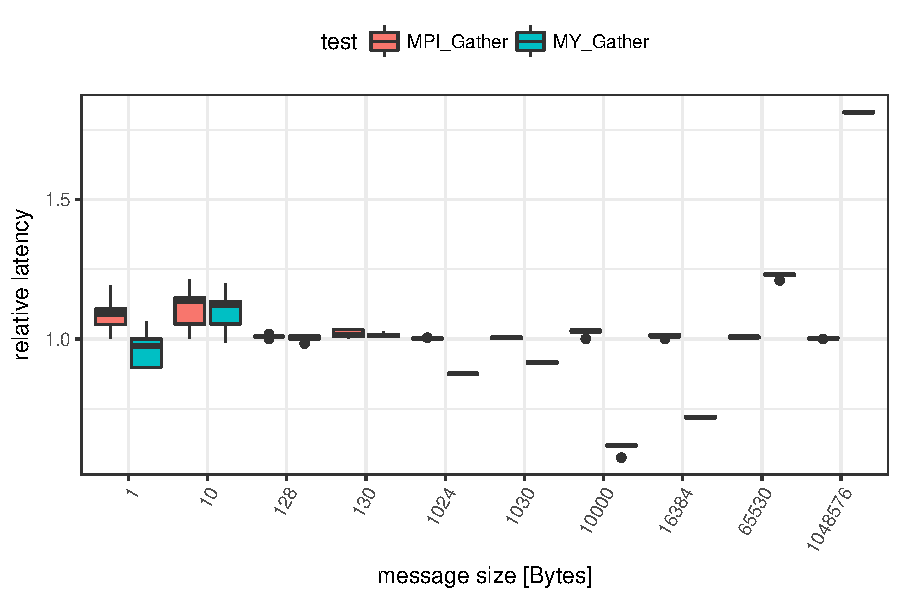
\includegraphics[width=\textwidth]{../benchmarks/openmpi/binom/gather_32/rel_runtime.pdf}
        \caption{Relative Runtime with $p=32 \times 16$}
        \label{fig:Gather:OpenMPI:Rel:32}
    \end{subfigure}
    \begin{subfigure}[b]{0.49\textwidth}
        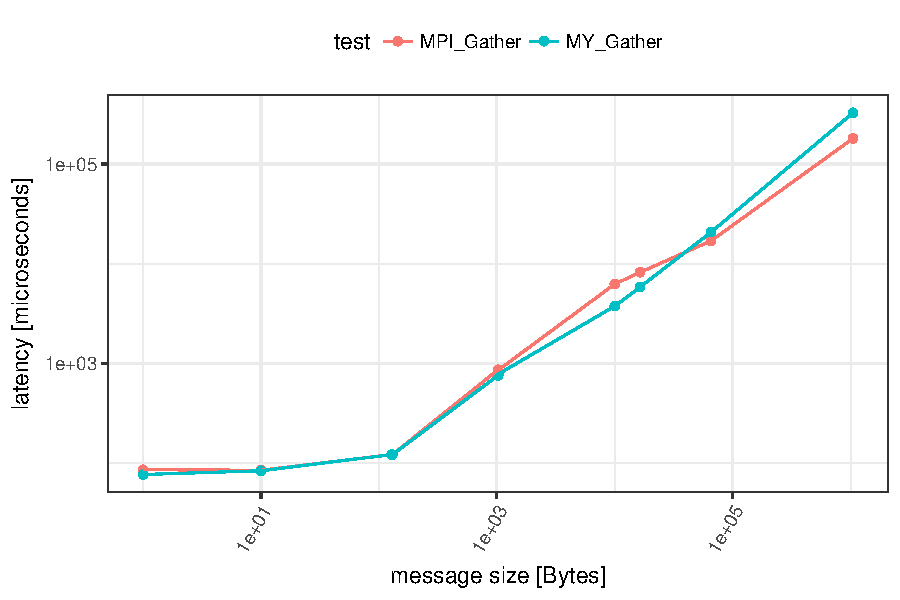
\includegraphics[width=\textwidth]{../benchmarks/openmpi/binom/gather_32/runtime.pdf}
        \caption{Absolute Runtime with $p=32 \times 16$}
        \label{fig:Gather:OpenMPI:Abs:32}
    \end{subfigure}
    
    \caption{\mygather compared to \mpigather of \texttt{Open MPI 1.10.3}}
\end{figure}

In both test cases, either with $512$ or with $496$ processes the implementations of \mygather and \mpigather (\texttt{Open MPI 1.10.3}) perform similarly in most of the cases. 
But with message sizes $> 100$ KByte the \mpigather implementation outperforms \mygather. We assume \mpigather implements some optimizations when dealing with big message sizes.

\begin{figure}[H]
    \centering
    
    \begin{subfigure}[b]{0.49\textwidth}
        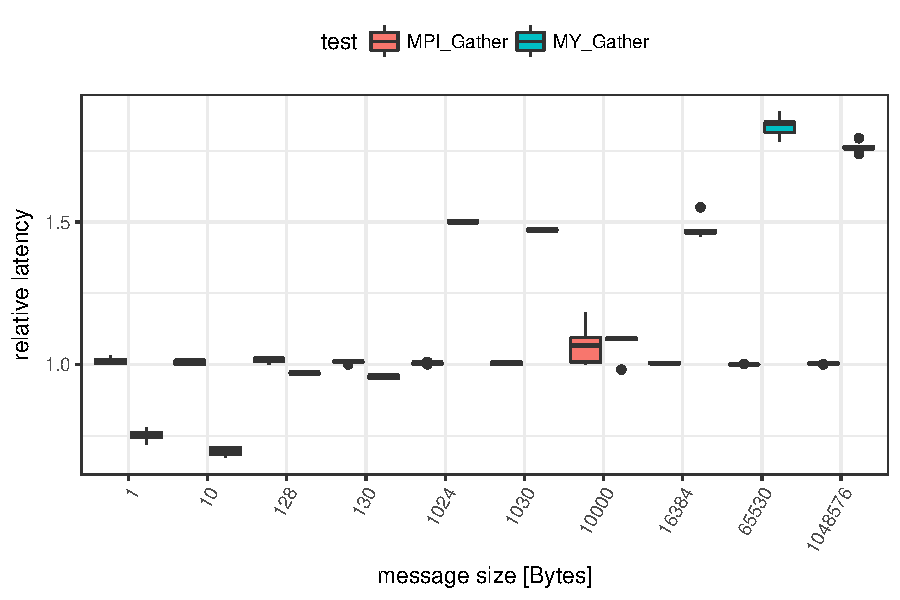
\includegraphics[width=\textwidth]{../benchmarks/mpich/binom/gather_31/rel_runtime.pdf}
        \caption{Relative Runtime with $p=31 \times 16$}
        \label{fig:Gather:MPICH:Rel:31}
    \end{subfigure}
    \begin{subfigure}[b]{0.49\textwidth}
        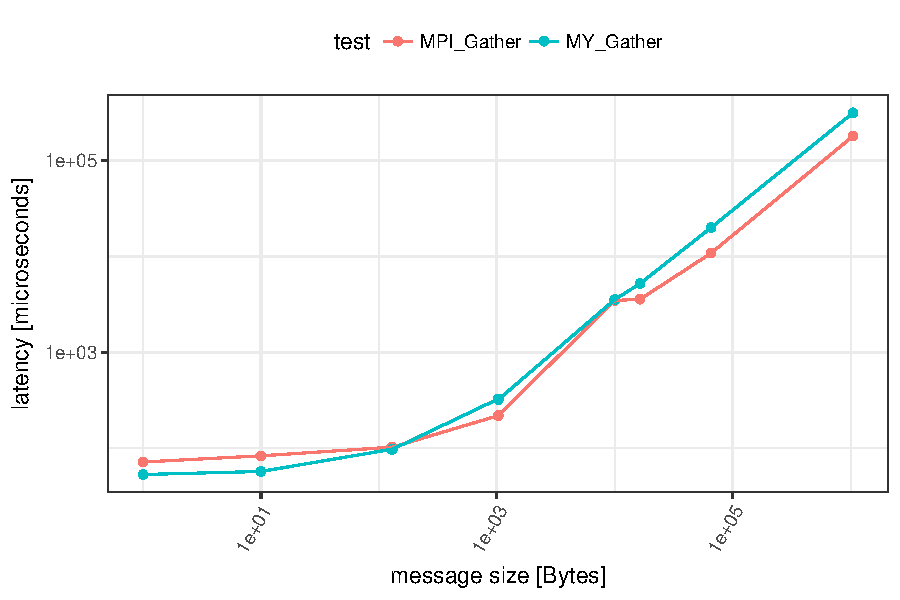
\includegraphics[width=\textwidth]{../benchmarks/mpich/binom/gather_31/runtime.pdf}
        \caption{Absolute Runtime with $p=31 \times 16$}
        \label{fig:Gather:MPICH:Abs:31}
    \end{subfigure}
    
    \begin{subfigure}[b]{0.49\textwidth}
        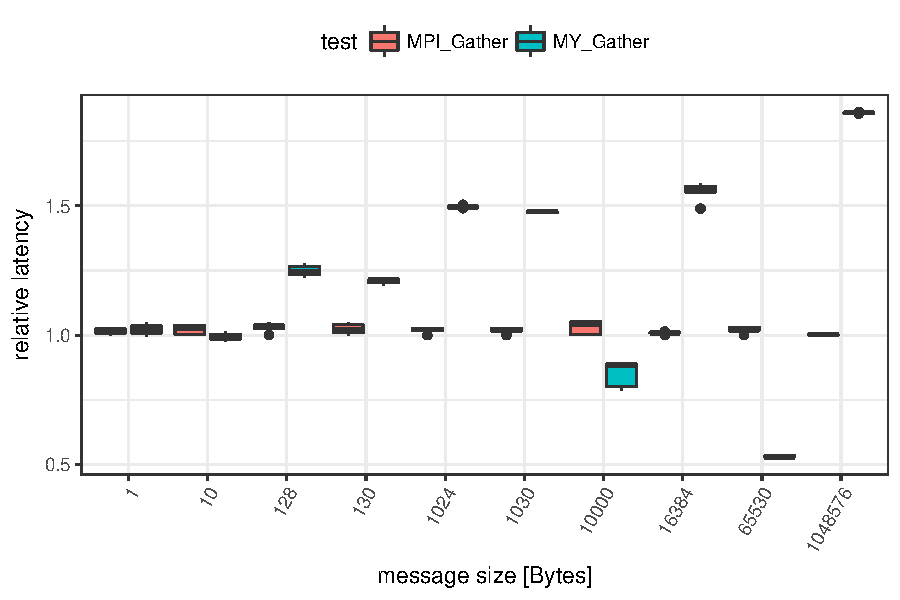
\includegraphics[width=\textwidth]{../benchmarks/mpich/binom/gather_32/rel_runtime.pdf}
        \caption{Relative Runtime with $p=32 \times 16$}
        \label{fig:Gather:MPICH:Rel:32}
    \end{subfigure}
    \begin{subfigure}[b]{0.49\textwidth}
        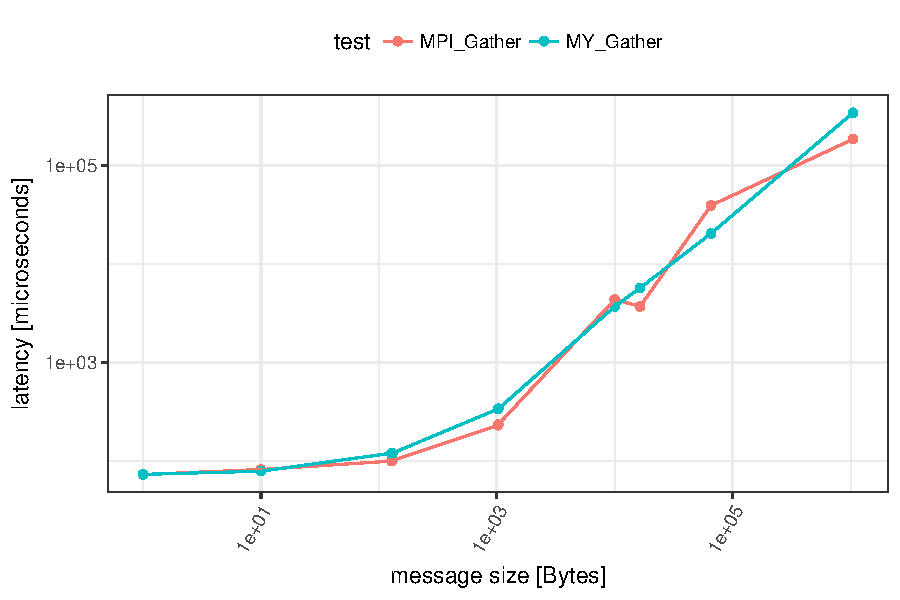
\includegraphics[width=\textwidth]{../benchmarks/mpich/binom/gather_32/runtime.pdf}
        \caption{Absolute Runtime with $p=32 \times 16$}
        \label{fig:Gather:MPICH:Abs:32}
    \end{subfigure}
    
    \caption{\mygather compared to \mpigather of \texttt{MVAPICH2 2.2}}
\end{figure}

\noindent Compared to the benchmark results before, the \mpigather implementation of \texttt{MVAPICH2 2.2} also slightly outperforms the \mygather implementations with smaller message sizes. The rather big latency changes when the message size exceeds $10$ KByte is also quite interesting, we assume that \texttt{MVAPICH2 2.2} switches to another algorithm when reaching a certain threshold.

%-------
\subsection{Experiments and Discussion -- \myscatter}

\begin{figure}[H]
    \centering
    
    \begin{subfigure}[b]{0.49\textwidth}
        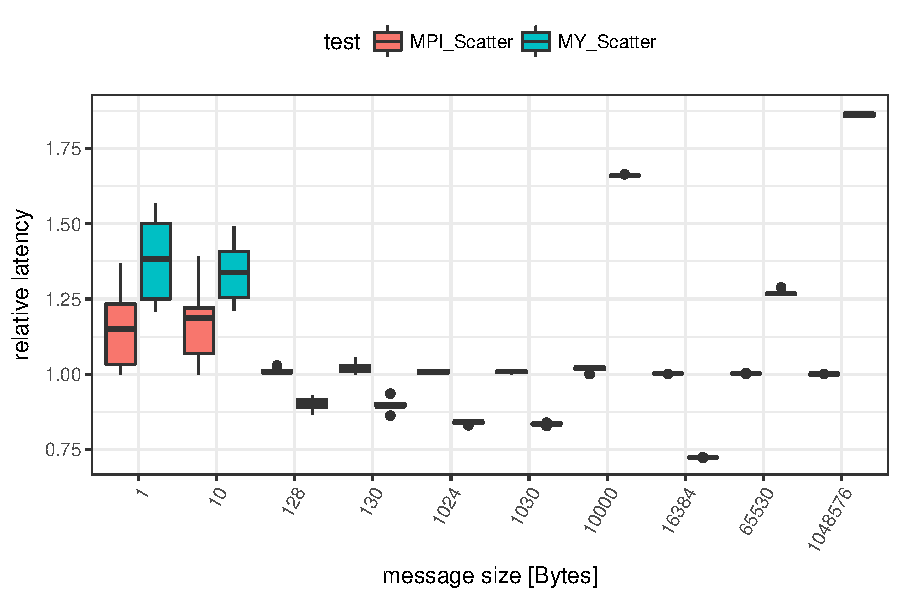
\includegraphics[width=\textwidth]{../benchmarks/openmpi/divide_conquer/scatter_31/rel_runtime.pdf}
        \caption{Relative Runtime with $p=31 \times 16$}
        \label{fig:Scatter:OpenMPI:Rel:31}
    \end{subfigure}
    \begin{subfigure}[b]{0.49\textwidth}
        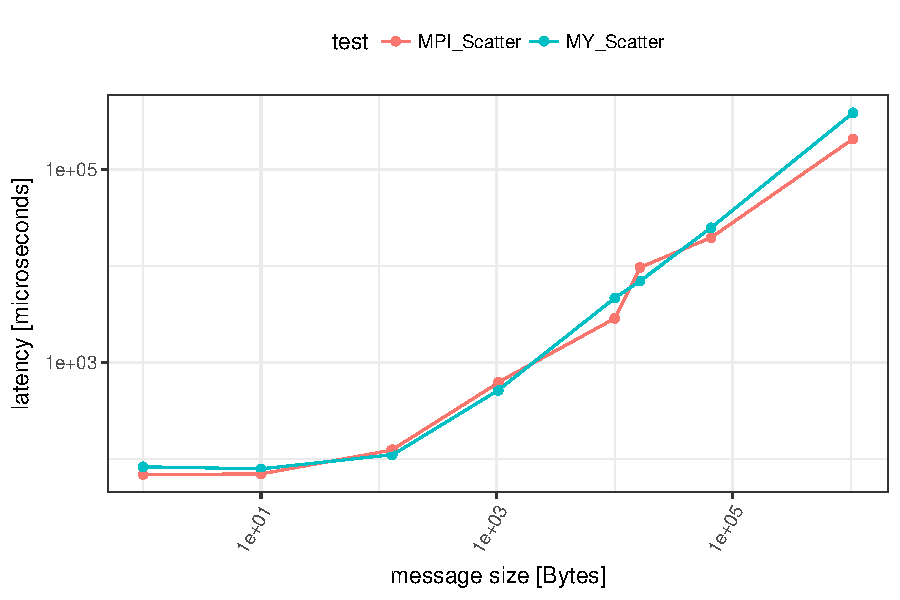
\includegraphics[width=\textwidth]{../benchmarks/openmpi/divide_conquer/scatter_31/runtime.pdf}
        \caption{Absolute Runtime with $p=31 \times 16$}
        \label{fig:Scatter:OpenMPI:Abs:31}
    \end{subfigure}
    
    \begin{subfigure}[b]{0.49\textwidth}
        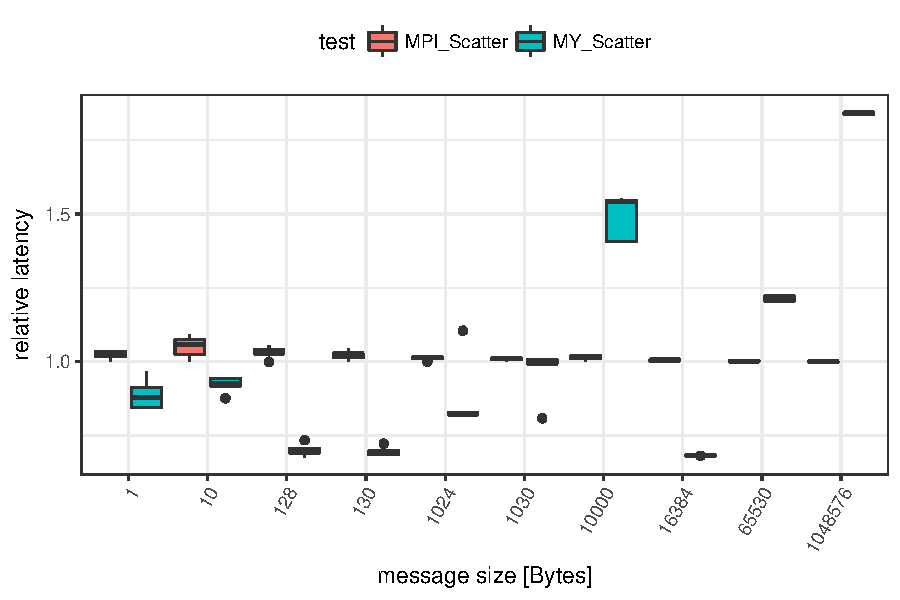
\includegraphics[width=\textwidth]{../benchmarks/openmpi/divide_conquer/scatter_32/rel_runtime.pdf}
        \caption{Relative Runtime with $p=32 \times 16$}
        \label{fig:Scatter:OpenMPI:Rel:32}
    \end{subfigure}
    \begin{subfigure}[b]{0.49\textwidth}
        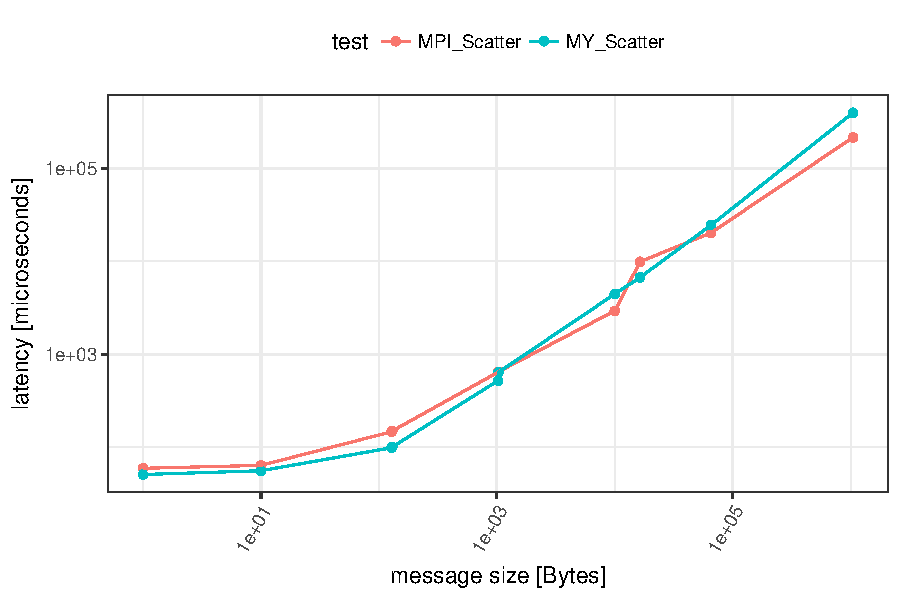
\includegraphics[width=\textwidth]{../benchmarks/openmpi/divide_conquer/scatter_32/runtime.pdf}
        \caption{Absolute Runtime with $p=32 \times 16$}
        \label{fig:Scatter:OpenMPI:Abs:32}
    \end{subfigure}
    
    \caption{\myscatter compared to \mpiscatter of \texttt{Open MPI 1.10.3}}
\end{figure}

Compared to the \texttt{Open MPI 1.10.3} implementation of \mpiscatter, \myscatter achieves similar performance for smaller message sizes. 
For bigger message sizes \mpiscatter outperforms \myscatter, which is again assumed to be because of optimizations for bigger messages.
We haven't found a reason for the particular widespread latency distribution of \myscatter when the message size is $10$ kByte, as seen in Figure \ref{fig:Scatter:OpenMPI:Rel:32}. 


\begin{figure}[H]
    \centering
    
    \begin{subfigure}[b]{0.49\textwidth}
        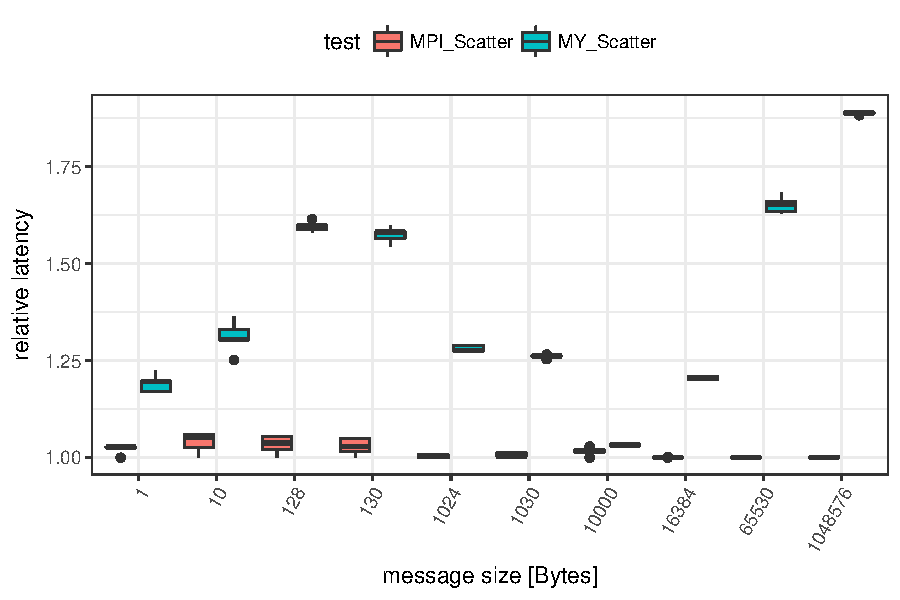
\includegraphics[width=\textwidth]{../benchmarks/mpich/divide_conquer/scatter_31/rel_runtime.pdf}
        \caption{Relative Runtime with $p=31 \times 16$}
        \label{fig:Scatter:MPICH:Rel:31}
    \end{subfigure}
    \begin{subfigure}[b]{0.49\textwidth}
        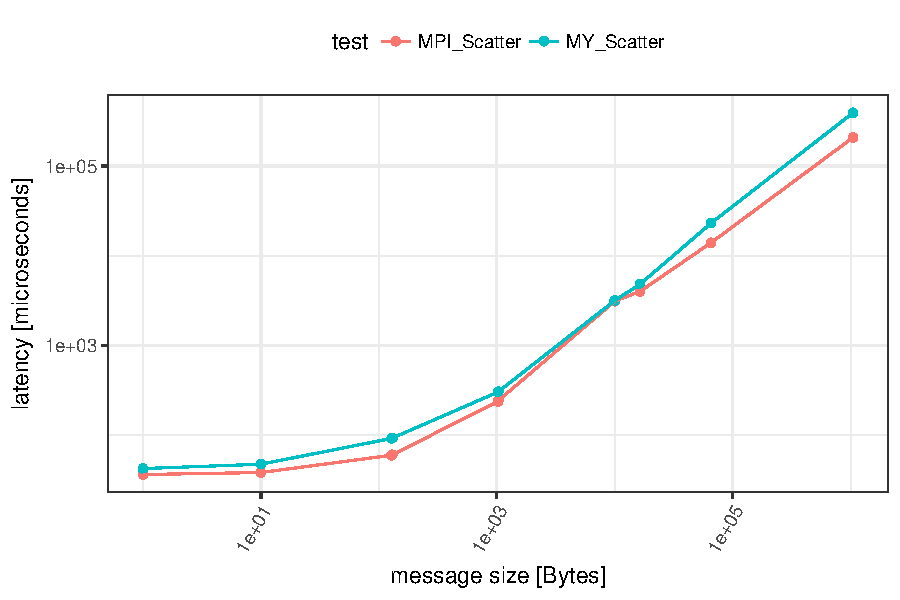
\includegraphics[width=\textwidth]{../benchmarks/mpich/divide_conquer/scatter_31/runtime.pdf}
        \caption{Absolute Runtime with $p=31 \times 16$}
        \label{fig:Scatter:MPICH:Abs:31}
    \end{subfigure}
    
    \begin{subfigure}[b]{0.49\textwidth}
        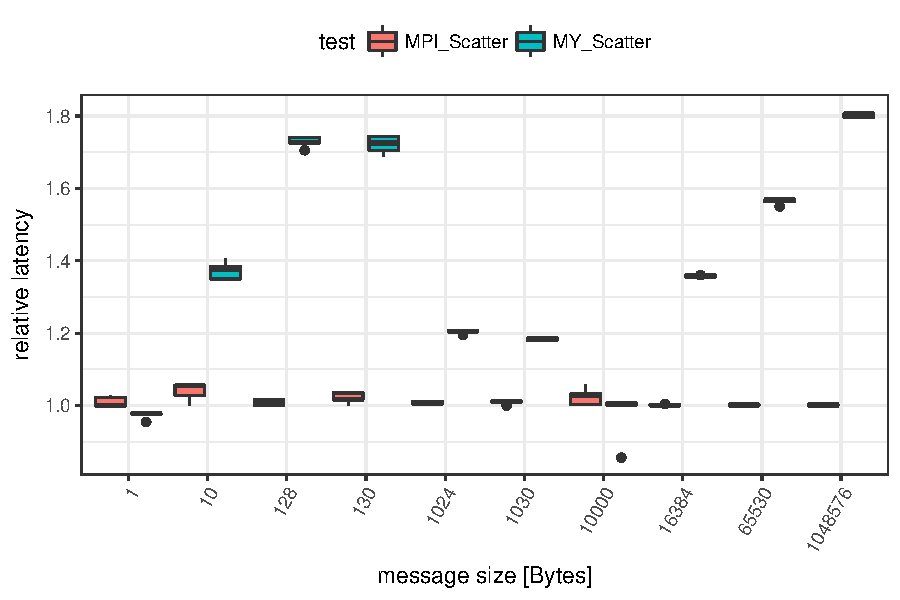
\includegraphics[width=\textwidth]{../benchmarks/mpich/divide_conquer/scatter_32/rel_runtime.pdf}
        \caption{Relative Runtime with $p=32 \times 16$}
        \label{fig:Scatter:MPICH:Rel:32}
    \end{subfigure}
    \begin{subfigure}[b]{0.49\textwidth}
        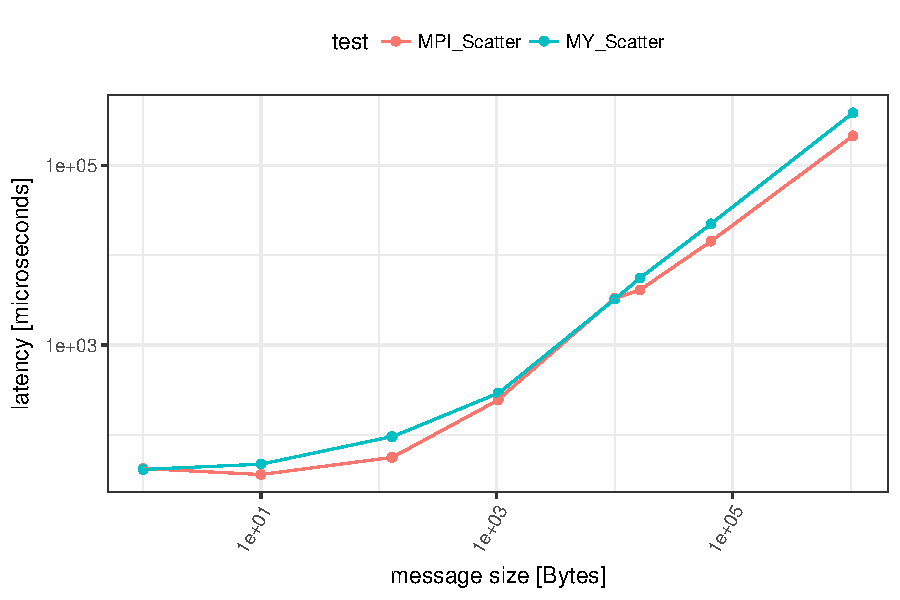
\includegraphics[width=\textwidth]{../benchmarks/mpich/divide_conquer/scatter_32/runtime.pdf}
        \caption{Absolute Runtime with $p=32 \times 16$}
        \label{fig:Scatter:MPICH:Abs:32}
    \end{subfigure}
    
    \caption{\myscatter compared to \mpiscatter of \texttt{MVAPICH2 2.2}}
\end{figure}

\noindent The \texttt{MVAPICH2 2.2} implementation of \mpigather outperforms \mygather in nearly all cases. The rather big latency changes when the message size exceeds $10$ KByte is also quite interesting, we assume that \texttt{MVAPICH2 2.2} switches to another algorithm when reaching a certain threshold.



% bibliography if needed, comment out if not needed
%\cleardoublepage
%\bibliographystyle{plainnat}
%\bibliography{myreferences}

\end{document}